\documentclass[11pt, oneside]{article}   	% use "amsart" instead of "article" for AMSLaTeX format
\usepackage{geometry}                		% See geometry.pdf to learn the layout options. There are lots.
\geometry{letterpaper}                   		% ... or a4paper or a5paper or ... 
%\geometry{landscape}                		% Activate for rotated page geometry
%\usepackage[parfill]{parskip}    		% Activate to begin paragraphs with an empty line rather than an indent
\usepackage{graphicx}				% Use pdf, png, jpg, or eps§ with pdflatex; use eps in DVI mode
								% TeX will automatically convert eps --> pdf in pdflatex		
\usepackage{amssymb}
\graphicspath{{.}}
\usepackage[document]{ragged2e}
\addtolength{\oddsidemargin}{-.875in}
	\addtolength{\evensidemargin}{-.875in}
	\addtolength{\textwidth}{1.75in}

	\addtolength{\topmargin}{-.875in}
	\addtolength{\textheight}{1.75in}
%SetFonts

%SetFonts*3


\title{Brief Article}
\author{The Author}
%\date{}							% Activate to display a given date or no date

\begin{document}
%\maketitle
%\section{}
%\subsection{}
\begin{flushright}
Donovan Guelde\\
CSCI 5622\\
logreg HW\\
\end{flushright}

1.  Final accuracy of the SGA implementaion increased rapidly from very small eta values, until a levelling-off at approximately eta=0.001.  This accuracy held in the range of eta = [0.001,1], but once eta grew past 1, accuracy decreased.  Low accuracy of very small eta values may reflect a learning step that was too small to climb the gradient to a maximum value in the number of runs completed, and decreased accuracy of large eta values may be due to continuous overshoot of the max.\\
\center
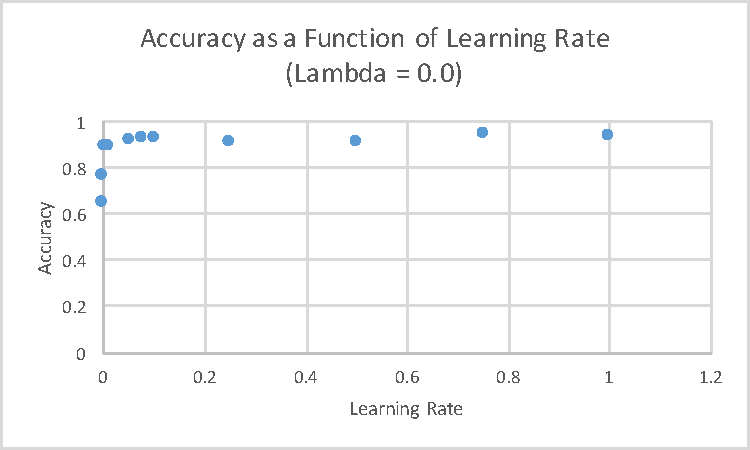
\includegraphics[totalheight=1.5in]{Picture1}
\justify
2.  Assuming that the gradient we are ascending is given by a convex function, a relatively large learning rate can be used in the early iterations, and steadily decreased as iterations continue, until the change in $P(y=1|x_i,D)$  from one iteration to the next is smaller than a predetermined limit.\\
\\
3,4.  To determine best (and worst) predictors, I calculated the change in odds of a sample being classified as y=1, based on adding one more instance of a given word.  The five highest and lowest predictors, and corresponding weights and odds changes, were:\\\\
\begin{tabular}{*3{c}}\hline
Word & weight (w) & resulting odds change (exp(w))\\ \hline
hit & 1.61504677899 & 5.02812312851 \\
pitching & 1.40274087306 & 4.06633000124 \\
baseball & 1.30444455192 & 3.68564134265 \\
runs & 1.27369921464 & 3.57404931405 \\
better & 1.08832236219 & 2.96928850109 \\
pts & -6.28964736324 & 0.00185541411873 \\
period & -2.29188370521 & 0.101075885243 \\
hockey & -2.24173937575 & 0.106273493986 \\
vs & -2.12459227351 & 0.119481674181 \\
shots & -1.99187415812 & 0.136439476524 \\
\end{tabular}
\\
\\
The following predictors had no effect on final classification (w=0, exp(w) = 1):\\
aggravatingly, alway, baby, contained, crumbled, favour, pronunciation, prototypical, ratio, sportscasters.


\end{document}  